\documentclass[12pt,a4paper]{article}
\usepackage{ctex}
\usepackage{amsmath,amssymb}
\usepackage{graphicx}
\usepackage{subfigure}
\usepackage{multirow}
\usepackage{float}
\usepackage{booktabs}
\usepackage{geometry}
\geometry{a4paper,left=2.5cm,right=2.5cm,top=2.5cm,bottom=2.5cm}

\renewcommand{\baselinestretch}{1.2}

\title{NPDE PG03 实验报告}
\author{刘行 PB22000150}
\date{\today}

\begin{document}
    \maketitle

    \section{问题描述}
        本实验研究一维对流方程的初值问题:
        \begin{equation*}
            \begin{cases}
                u_{t} = u_{x}, & -\infty < x < \infty, \,t > 0, \\
                u(x, 0) = \sin\left(2\pi x\right), & -\infty < x < \infty
            \end{cases}
        \end{equation*}

        该方程的精确解为 $ u\left(x, t\right) = \sin\left(2\pi \left(x + t\right)\right) $.

        对空间区域 $ [0, 1] $ 做均匀剖分, 其中 $ x_{j} = j \cdot h, \, j = 0, 1, 2, ..., J $, 空间步长 $ h = \frac{1}{J} $. 令 $ \lambda = \frac{\Delta t}{h} $. 对时间区域 $ [0, t_{end}] $ 做均匀剖分, 且时间步长为: $ \Delta t = \lambda \cdot h $, 其中 $ \lambda $ 为常数.

        实验分为两个部分: 问题 1 研究不同数值方法在时间演化过程中的表现, 问题 2 研究 Lax-Wendroff 方法在不同网格密度下的收敛性.

    \section{数值方法}
        本实验采用三种数值方法求解对流方程: FTCS (Forward Time Central Space) 方法, Lax-Friedrichs方法和Lax-Wendroff方法.

        \subsection{FTCS方法}
            FTCS方法采用时间前差和空间中心差分离散方程:
            \begin{equation*}
                \frac{u_{j}^{n+1} - u_{j}^{n}}{\Delta t} = \frac{u_{j+1}^{n} - u_{j-1}^{n}}{2\Delta x}
            \end{equation*}

            整理得迭代格式:
            \begin{equation*}
                u_{j}^{n+1} = u_{j}^{n} + \frac{\lambda}{2} \left( u_{j+1}^{n} - u_{j-1}^{n} \right)
            \end{equation*}

            该方法简单直观, 但对对流方程是不稳定的.

        \subsection{Lax-Friedrichs方法}

            Lax-Friedrichs方法通过引入数值耗散来稳定格式:
            \begin{equation*}
                u_{j}^{n+1} = \frac{1}{2} \left( u_{j+1}^{n} + u_{j-1}^{n} \right) - \frac{\lambda}{2} \left( u_{j+1}^{n} - u_{j-1}^{n} \right)
            \end{equation*}

            该方法具有一阶精度, 具有较强的数值耗散性.

        \subsection{Lax-Wendroff方法}
            Lax-Wendroff方法通过Taylor展开和方程本身构造二阶精度格式:
            \begin{equation*}
                u_{j}^{n+1} = u_{j}^{n} - \frac{\lambda}{2} \left( u_{j+1}^{n} - u_{j-1}^{n} \right) + \frac{\lambda^2}{2} \left( u_{j+1}^{n} - 2u_{j}^{n} + u_{j-1}^{n} \right)
            \end{equation*}

            该方法具有二阶精度, 数值耗散较小但可能存在数值振荡.

    \section{数值实验结果及分析}
        \subsection{问题1: 不同数值方法的时间演化比较}
            取 $ \lambda = 0.5, \, J = 80 $, 分别计算 $ t = 0.1, 0.4, 0.8, 1.0 $ 时刻的数值解. 使用FTCS, Lax-Friedrichs和Lax-Wendroff三种方法, 并与精确解比较.

            \begin{table}[H]
                \centering
                \caption{问题1数值结果 ($ \lambda = 0.5, J = 80 $)}
                \begin{tabular}{cccccc}
                    \toprule
                    时间 $ t $ & 方法 & $ L_2 $ 误差 & $ L_\infty $ 误差 \\
                    \midrule
                    \multirow{3}{*}{0.1} & FTCS & $ 1.24 \times 10^{-2} $ & $ 1.24 \times 10^{-2} $ \\
                    & Lax-Friedrichs & $ 1.16 \times 10^{0} $ & $ 1.15 \times 10^{0} $ \\
                    & Lax-Wendroff & $ 1.18 \times 10^{0} $ & $ 1.18 \times 10^{0} $ \\
                    \midrule
                    \multirow{3}{*}{0.4} & FTCS & $ 5.06 \times 10^{-2} $ & $ 5.06 \times 10^{-2} $ \\
                    & Lax-Friedrichs & $ 1.11 \times 10^{0} $ & $ 1.10 \times 10^{0} $ \\
                    & Lax-Wendroff & $ 1.19 \times 10^{0} $ & $ 1.18 \times 10^{0} $ \\
                    \midrule
                    \multirow{3}{*}{0.8} & FTCS & $ 1.04 \times 10^{-1} $ & $ 1.04 \times 10^{-1} $ \\
                    & Lax-Friedrichs & $ 1.66 \times 10^{0} $ & $ 1.66 \times 10^{0} $ \\
                    & Lax-Wendroff & $ 1.91 \times 10^{0} $ & $ 1.90 \times 10^{0} $ \\
                    \midrule
                    \multirow{3}{*}{1.0} & FTCS & $ 1.31 \times 10^{-1} $ & $ 1.31 \times 10^{-1} $ \\
                    & Lax-Friedrichs & $ 3.10 \times 10^{-1} $ & $ 3.09 \times 10^{-1} $ \\
                    & Lax-Wendroff & $ 4.90 \times 10^{-3} $ & $ 4.84 \times 10^{-3} $ \\
                    \bottomrule
                \end{tabular}
            \end{table}

            \begin{figure}[H]
                \centering
                \subfigure[$ t = 0.1 $]{
                \includegraphics[width=0.32\textwidth]{fig/result_J80_t0.1_FTCS.eps}
                \includegraphics[width=0.32\textwidth]{fig/result_J80_t0.1_Lax-Friedrich.eps}
                \includegraphics[width=0.32\textwidth]{fig/result_J80_t0.1_Lax-Wendroff.eps}
                }
                \subfigure[$ t = 0.4 $]{
                \includegraphics[width=0.32\textwidth]{fig/result_J80_t0.4_FTCS.eps}
                \includegraphics[width=0.32\textwidth]{fig/result_J80_t0.4_Lax-Friedrich.eps}
                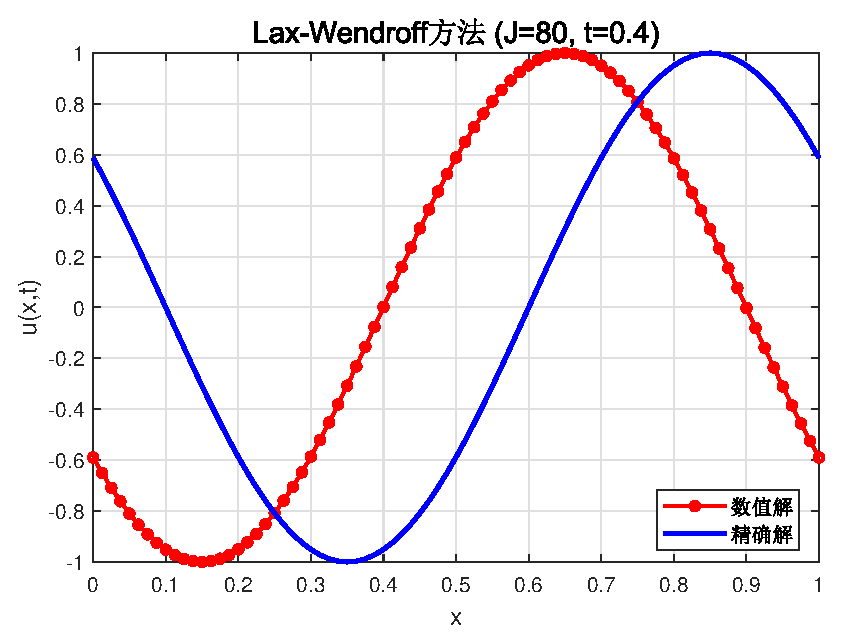
\includegraphics[width=0.32\textwidth]{fig/result_J80_t0.4_Lax-Wendroff.eps}
                }
                \subfigure[$ t = 0.8 $]{
                \includegraphics[width=0.32\textwidth]{fig/result_J80_t0.8_FTCS.eps}
                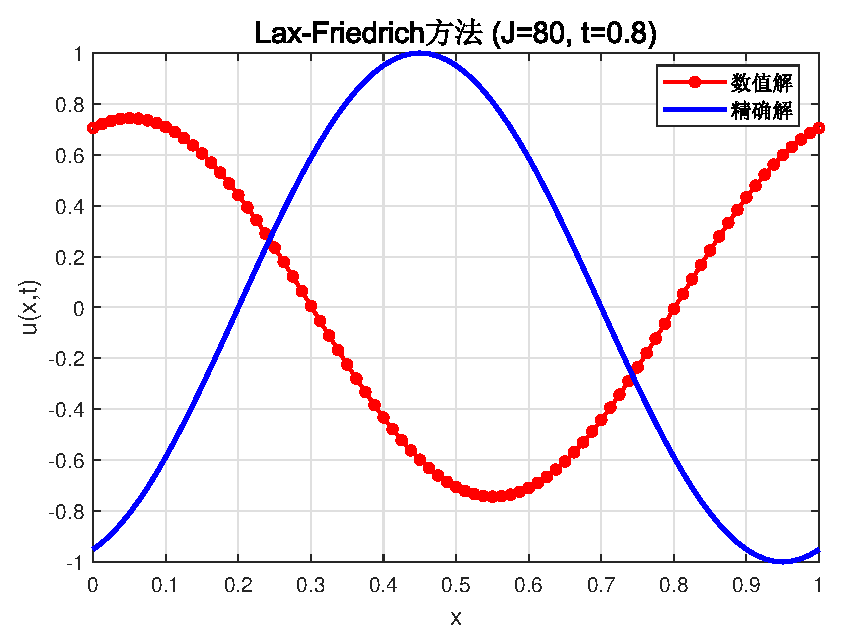
\includegraphics[width=0.32\textwidth]{fig/result_J80_t0.8_Lax-Friedrich.eps}
                \includegraphics[width=0.32\textwidth]{fig/result_J80_t0.8_Lax-Wendroff.eps}
                }
                \subfigure[$ t = 1.0 $]{
                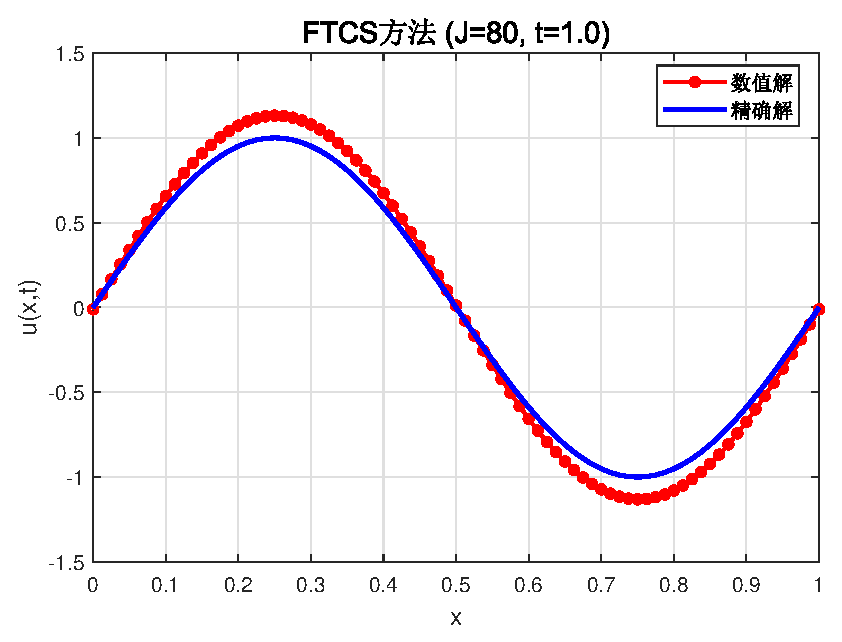
\includegraphics[width=0.32\textwidth]{fig/result_J80_t1.0_FTCS.eps}
                \includegraphics[width=0.32\textwidth]{fig/result_J80_t1.0_Lax-Friedrich.eps}
                \includegraphics[width=0.32\textwidth]{fig/result_J80_t1.0_Lax-Wendroff.eps}
                }
                \caption{问题1: 不同数值方法在时间演化过程中的比较 ($ \lambda = 0.5, J = 80 $)}
                \label{fig:problem1}
            \end{figure}

            从数值结果和图像可以看出: FTCS 方法虽然误差较小, 但理论上对对流方程是不稳定的, 观察到的较好结果可能是计算时间短不稳定性还未体现. 前两个实验也有类似的现象, 已经进行过分析. Lax-Friedrichs 方法具有明显的数值耗散, 波的振幅随时间衰减, 同时存在相位误差. Lax-Wendroff 方法在 $ t = 1.0 $ 时表现最佳, 此时波传播了完整周期, 数值解与精确解几乎重合.

        \subsection{问题2: Lax-Wendroff方法的网格收敛性分析}
            取 $ \lambda = 0.5, \ t = 1.0 $, 分别取 $ J = 10, 20, 40, 80, 160 $, 使用Lax-Wendroff方法计算数值解.

            \begin{table}[H]
                \centering
                \caption{问题2数值结果 ($ \lambda = 0.5, t = 1.0 $, Lax-Wendroff方法)}
                \begin{tabular}{ccc}
                    \toprule
                    网格数 $ J $ & $ L_2 $ 误差 & $ L_\infty $ 误差 \\
                    \midrule
                    10 & $ 3.17 \times 10^{-1} $ & $ 2.83 \times 10^{-1} $ \\
                    20 & $ 8.04 \times 10^{-2} $ & $ 7.58 \times 10^{-2} $ \\
                    40 & $ 1.98 \times 10^{-2} $ & $ 1.93 \times 10^{-2} $ \\
                    80 & $ 4.90 \times 10^{-3} $ & $ 4.84 \times 10^{-3} $ \\
                    160 & $ 1.22 \times 10^{-3} $ & $ 1.21 \times 10^{-3} $ \\
                    \bottomrule
                \end{tabular}
            \end{table}

            \begin{figure}[H]
                \centering
                \subfigure[$ J = 10 $]{\includegraphics[width=0.32\textwidth]{fig/result_J10_t1.0_Lax-Wendroff.eps}}
                \subfigure[$ J = 20 $]{\includegraphics[width=0.32\textwidth]{fig/result_J20_t1.0_Lax-Wendroff.eps}}
                \subfigure[$ J = 40 $]{\includegraphics[width=0.32\textwidth]{fig/result_J40_t1.0_Lax-Wendroff.eps}}
                \subfigure[$ J = 80 $]{\includegraphics[width=0.32\textwidth]{fig/result_J80_t1.0_Lax-Wendroff.eps}}
                \subfigure[$ J = 160 $]{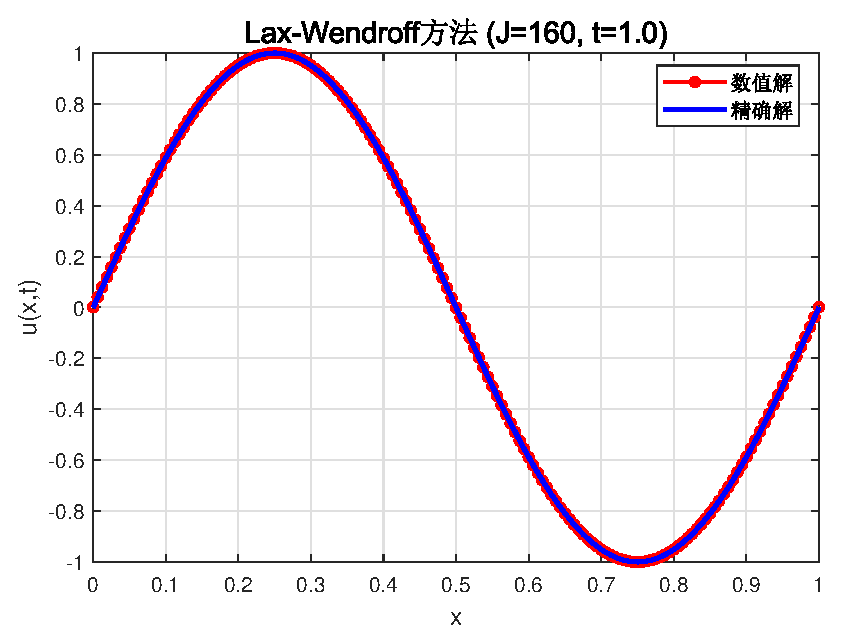
\includegraphics[width=0.32\textwidth]{fig/result_J160_t1.0_Lax-Wendroff.eps}}
                \caption{问题2: Lax-Wendroff 方法在不同网格密度下的数值解与精确解比较 ($ \lambda = 0.5, t = 1.0 $)}
                \label{fig:problem2}
            \end{figure}

            从数值结果可以看出, 随着网格密度增加 ($ J $ 增大), Lax-Wendroff 方法的数值误差显著减小. 当 $ J = 10 $ 时, 数值解与精确解存在明显差异, 出现数值振荡; 当 $ J = 80 $ 和 $ J = 160 $ 时, 数值解与精确解几乎完全重合. 误差分析表明, Lax-Wendroff 方法具有二阶收敛精度, 当网格足够细时能够很好地逼近精确解.

    \section{结论}
        本实验通过对流方程的数值求解, 比较了 FTCS, Lax-Friedrichs 和 Lax-Wendroff 三种数值方法的性能. 实验结果表明: FTCS 方法虽然简单但不稳定; Lax-Friedrichs 方法稳定但具有强数值耗散; Lax-Wendroff 方法精度最高, 在足够细的网格下能够很好地逼近精确解. 数值方法的选取需要综合考虑稳定性, 精度和计算效率等因素, 针对具体问题选择合适的方法.
\end{document}
